% ============================================================
\chapter{Motivations and Overview}
\label{ch:motivations}
% ============================================================

Imagine a point cloud in a high-dimensional space. Classical statistics will
give you its mean, its variance, its principal components. But they will not
tell you whether there is a ``hole'' in the middle, a loop, or two clusters
separated by a void. These \emph{topological} features --- the global shape
of the data --- are often the most informative. This is the founding
intuition of \emph{topological data analysis} (TDA), a field born in the
early 2000s from the work of Gunnar Carlsson, Herbert Edelsbrunner, and
others, at the frontier of algebraic topology, computational geometry, and
data science.

\begin{intuition}
Why do we need topology to analyze data? Because the \emph{shape} of
data --- its holes, connected components, and cavities --- carries
information that classical statistics cannot capture.
\end{intuition}

% ============================================================
\section{The Fundamental Problem}
% ============================================================

Consider a point cloud $X = \{x_1, \ldots, x_n\} \subset \R^d$. This
cloud is often a noisy sample from an underlying topological space
$\mathcal{M}$ (a manifold, curve, surface, etc.). The central problem
of TDA is:

\begin{keyformulas}[title=\textbf{Fundamental Question}]
\emph{How can we recover the topological properties of $\mathcal{M}$
from the finite sample $X$?}
\end{keyformulas}

\begin{example}
Let $\mathcal{M} = S^1$ be the unit circle in $\R^2$. A sample of
$100$ noisy points on this circle forms a ring. Topologically, $S^1$
has one connected component ($\beta_0 = 1$) and one hole ($\beta_1 = 1$).
TDA allows us to recover these invariants from the point cloud.
\end{example}

% ============================================================
\section{Limitations of Classical Approaches}
% ============================================================

Classical statistical and learning methods have several limitations when
dealing with data of complex shape:

\begin{enumerate}
  \item \textbf{Coordinate dependence}: descriptive statistics (mean,
        variance) depend on the chosen coordinate system. Topology is
        invariant under homeomorphism.
  \item \textbf{Loss of structural information}: clustering identifies
        connected components but ignores holes and cavities.
  \item \textbf{Curse of dimensionality}: in high dimensions, Euclidean
        distances become uninformative, but topological invariants remain
        meaningful.
  \item \textbf{Lack of multi-scale analysis}: fixing a distance
        threshold is arbitrary; persistence explores \emph{all} scales
        simultaneously.
\end{enumerate}

% ============================================================
\section{The Philosophy of TDA}
% ============================================================

TDA rests on three guiding principles:

\begin{definition}[Principles of TDA]
\begin{enumerate}
  \item \textbf{Deformation invariance}: topological properties are
        preserved under continuous deformation (homeomorphism, homotopy
        equivalence).
  \item \textbf{Multi-scale approach}: rather than fixing a resolution
        parameter, we study the evolution of topology across all
        resolution scales.
  \item \textbf{Stability}: small perturbations of the data produce
        small perturbations of the topological descriptors.
\end{enumerate}
\end{definition}

% ============================================================
\section{Visual Illustration: From Point Cloud to Complex}
% ============================================================

The fundamental construction of TDA consists of progressively thickening
a point cloud into a geometric object whose topology can be computed.

\begin{center}
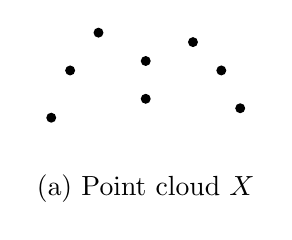
\begin{tikzpicture}[scale=1.2]
  % Points
  \foreach \p in {(0,0),(1,0.2),(0.5,0.9),(1.5,0.8),(2,0.1),
                  (0.2,0.5),(1.8,0.5),(1,0.6)}{
    \fill \p circle (1.5pt);
  }
  \node[below] at (1,-0.5) {(a) Point cloud $X$};
\end{tikzpicture}
\hspace{1cm}
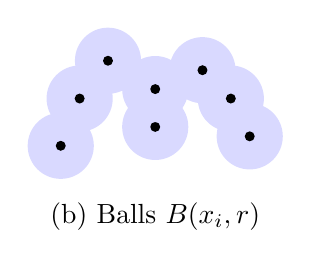
\begin{tikzpicture}[scale=1.2]
  % Points with balls
  \foreach \p in {(0,0),(1,0.2),(0.5,0.9),(1.5,0.8),(2,0.1),
                  (0.2,0.5),(1.8,0.5),(1,0.6)}{
    \fill[blue!15] \p circle (0.35);
    \fill \p circle (1.5pt);
  }
  \node[below] at (1,-0.5) {(b) Balls $B(x_i, r)$};
\end{tikzpicture}
\hspace{1cm}
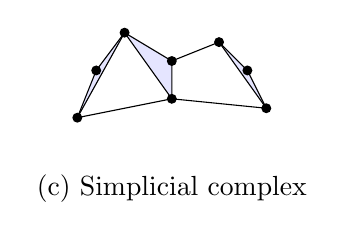
\begin{tikzpicture}[scale=1.2]
  % Simplicial complex
  \fill[blue!10] (0,0) -- (0.2,0.5) -- (0.5,0.9) -- cycle;
  \fill[blue!10] (0.5,0.9) -- (1,0.6) -- (1,0.2) -- cycle;
  \fill[blue!10] (1.5,0.8) -- (1.8,0.5) -- (2,0.1) -- cycle;
  \draw (0,0) -- (1,0.2) -- (0.5,0.9) -- cycle;
  \draw (0,0) -- (0.2,0.5) -- (0.5,0.9);
  \draw (1,0.2) -- (1,0.6) -- (1.5,0.8);
  \draw (1,0.6) -- (0.5,0.9);
  \draw (1.5,0.8) -- (1.8,0.5) -- (2,0.1);
  \draw (1,0.2) -- (2,0.1);
  \draw (1.5,0.8) -- (2,0.1);
  \foreach \p in {(0,0),(1,0.2),(0.5,0.9),(1.5,0.8),(2,0.1),
                  (0.2,0.5),(1.8,0.5),(1,0.6)}{
    \fill \p circle (1.5pt);
  }
  \node[below] at (1,-0.5) {(c) Simplicial complex};
\end{tikzpicture}
\end{center}

% ============================================================
\section{Betti Numbers: A First Intuition}
% ============================================================

Betti numbers are the simplest topological invariants. Intuitively:

\begin{keyformulas}[title=\textbf{Betti Numbers}]
\begin{align}
\beta_0 &= \text{number of connected components} \\
\beta_1 &= \text{number of holes (loops)} \\
\beta_2 &= \text{number of cavities (enclosed voids)} \\
\beta_p &= \text{number of ``holes'' of dimension } p
\end{align}
\end{keyformulas}

\begin{example}
\begin{itemize}
  \item A filled disk: $\beta_0 = 1$, $\beta_1 = 0$.
  \item A circle $S^1$: $\beta_0 = 1$, $\beta_1 = 1$.
  \item A torus $T^2$: $\beta_0 = 1$, $\beta_1 = 2$, $\beta_2 = 1$.
  \item A sphere $S^2$: $\beta_0 = 1$, $\beta_1 = 0$, $\beta_2 = 1$.
\end{itemize}
\end{example}

% ============================================================
\section{A Typical TDA Pipeline}
% ============================================================

The general topological analysis process follows these steps:

\begin{algorithme}[title=\textbf{Standard TDA Pipeline}]
\begin{enumerate}
  \item \textbf{Data}: point cloud $X \subset \R^d$ or distance matrix.
  \item \textbf{Filtration}: build a nested family of simplicial
        complexes $K_{r_1} \subseteq K_{r_2} \subseteq \cdots$.
  \item \textbf{Persistent homology}: compute the birth and death of
        each topological feature.
  \item \textbf{Representation}: encode the result as a persistence
        diagram or barcode.
  \item \textbf{Vectorization}: transform into a feature vector for
        learning.
  \item \textbf{Analysis/Prediction}: apply statistical or ML methods.
\end{enumerate}
\end{algorithme}

\begin{codeblock}[title=\textbf{First Example with Ripser}]
\begin{minted}{python}
import numpy as np
from ripser import ripser
import matplotlib.pyplot as plt
from persim import plot_diagrams

# Generate a noisy circle
theta = np.linspace(0, 2*np.pi, 100, endpoint=False)
X = np.column_stack([np.cos(theta), np.sin(theta)])
X += 0.1 * np.random.randn(*X.shape)

# Compute persistent homology
result = ripser(X, maxdim=1)
diagrams = result['dgms']

# Visualize
fig, axes = plt.subplots(1, 2, figsize=(12, 5))
axes[0].scatter(X[:, 0], X[:, 1], s=10)
axes[0].set_title("Point Cloud")
axes[0].set_aspect('equal')
plot_diagrams(diagrams, ax=axes[1])
axes[1].set_title("Persistence Diagram")
plt.tight_layout()
plt.savefig("first_tda_example.pdf")
\end{minted}
\end{codeblock}

% ============================================================
\section{Overview of Applications}
% ============================================================

TDA has demonstrated its usefulness across many domains:

\subsection{Biology and Medicine}
\begin{itemize}
  \item \textbf{Protein shape analysis}: persistent Betti numbers
        characterize cavities and tunnels in molecular structures.
  \item \textbf{Genomics}: Mapper reveals subgroups in breast cancer
        gene expression data.
  \item \textbf{Medical imaging}: tumor detection via persistent
        homology of images.
\end{itemize}

\subsection{Neuroscience}
\begin{itemize}
  \item \textbf{Brain connectome}: topological analysis of neural
        networks.
  \item \textbf{Neural codes}: persistent homology reveals the
        structure of spatial representations (place cells).
\end{itemize}

\subsection{Materials Science}
\begin{itemize}
  \item \textbf{Amorphous materials}: characterization of medium-range
        order.
  \item \textbf{Porous materials}: porosity quantification via Betti
        numbers.
\end{itemize}

\subsection{Time Series and Signals}
\begin{itemize}
  \item \textbf{Anomaly detection}: topological changes signal
        abnormal regimes.
  \item \textbf{Takens reconstruction}: embedding a time series and
        analyzing the resulting shape.
\end{itemize}

% ============================================================
\section{Mathematical Formalism: A First Glimpse}
% ============================================================

We conclude this introductory chapter with a formal overview of the
main objects, which will be developed in subsequent chapters.

\begin{definition}[Filtration]
A \emph{filtration} is a family of topological subspaces (or simplicial
complexes) $\{K_r\}_{r \in \R}$ such that:
\[
  r \leq s \implies K_r \subseteq K_s.
\]
\end{definition}

\begin{definition}[Persistence Module]
A \emph{persistence module} is a functor
$\mathbf{V} : (\R, \leq) \to \mathbf{Vec}_\mathbb{F}$ that assigns to
each $r \in \R$ a vector space $V_r$ and to each pair $r \leq s$ a
linear map $v_r^s : V_r \to V_s$.
\end{definition}

\begin{theorem}[Decomposition of Persistence Modules]
Every \emph{pointwise finite-dimensional} (p.f.d.) persistence module
decomposes uniquely (up to isomorphism) as a direct sum of interval
modules:
\[
  \mathbf{V} \cong \bigoplus_{j \in J} \mathbb{I}[b_j, d_j)
\]
where $\mathbb{I}[b,d)$ is the module that equals $\mathbb{F}$ on
$[b,d)$ and $0$ elsewhere, with identity maps on the interval.
\end{theorem}

% ============================================================
\section{Why Topology and Not Just Geometry?}
% ============================================================

\begin{remark}
Geometry studies metric properties (distances, curvatures, angles) that
depend on the embedding. Topology studies properties invariant under
continuous deformation: it is coarser but more robust. TDA exploits
this robustness to extract essential information.

For instance, a coffee mug and a donut are topologically identical
(both have one hole), even though they are geometrically very different.
\end{remark}

% ============================================================
\section{Exercises}
% ============================================================

\begin{exercise}
Generate a cloud of $200$ points sampled uniformly on a torus in $\R^3$
(standard parametrization with $R=2, r=1$). Add Gaussian noise with
variance $\sigma^2 = 0.05$. Compute persistent homology with
\texttt{ripser} and verify that you recover $\beta_0 = 1$,
$\beta_1 = 2$, $\beta_2 = 1$.
\end{exercise}

\begin{exercise}
Explain why Betti numbers alone are not sufficient to distinguish all
topological spaces. Give an example of two spaces with the same Betti
numbers that are not homeomorphic.
\end{exercise}

\begin{exercise}
Implement the naive computation of the pairwise distance matrix for a
cloud of $n$ points in $\R^d$. What is the complexity? How is this
matrix used in the construction of a Vietoris--Rips complex?
\end{exercise}

\begin{exercise}
Find a recent paper (post-2020) using TDA in an application domain of
your choice. Summarize the methodology in one page: what data, which
complex, which topological descriptors, what main result?
\end{exercise}
